\section{Paralelismo en Python}

\begin{frame}{El GIL y sus efectos}
  \begin{itemize}
    \item El Global Interpreter Lock protege el conteo de referencias, permitiendo un único hilo de bytecode a la vez.
    \item En tareas CPU los hilos compiten por el GIL y pueden ser más lentos que la versión secuencial.
    \item El intérprete libera el GIL durante E/S bloqueante, por lo que el modelo sigue siendo útil para cargas I/O-bound.
  \end{itemize}
\end{frame}

\begin{frame}{Threading para E/S}
  \begin{itemize}
    \item Ideal para servidores que esperan red o disco; la latencia se oculta mientras otros hilos avanzan.
    \item Sin paralelismo real en CPU intensivo; evite usarlo para cómputo pesado.
    \item Coordine con colas o semáforos de la librería estándar para evitar condiciones de carrera en datos compartidos.
  \end{itemize}
\end{frame}

\begin{frame}[fragile]{Multiprocessing: evasión del GIL}
  \lstset{language=Python}
  \begin{lstlisting}
from multiprocessing import Pool, cpu_count

def cpu_intensive_task(n):
    return n * n

if __name__ == '__main__':
    with Pool(processes=cpu_count()) as pool:
        results = pool.map(cpu_intensive_task, range(8))
  \end{lstlisting}
  \begin{itemize}
    \item Cada proceso tiene su propio intérprete y GIL; se paga serialización de datos (pickle) e IPC.
    \item Usar bloques \texttt{if \_\_name\_\_ == '\_\_main\_\_'} evita creación recursiva de procesos en Windows.
  \end{itemize}
\end{frame}

\begin{frame}[fragile]{Joblib para ciencia de datos}
  \lstset{language=Python}
  \begin{lstlisting}
from joblib import Parallel, delayed

def process_image_stub(image_id):
    return f'Img {image_id} done'

results = Parallel(
    n_jobs=-1, prefer='processes', verbose=5
)(delayed(process_image_stub)(i) for i in range(20))
  \end{lstlisting}
  \begin{itemize}
    \item Sintaxis declarativa para pipelines intensivos en CPU; \texttt{n\_jobs=-1} usa todos los núcleos.
    \item Puede usar \texttt{memmap} para compartir arrays grandes sin copias, reduciendo la sobrecarga de pickle.
  \end{itemize}
\end{frame}

\begin{frame}{Visual del GIL}
  \begin{figure}
    \centering
    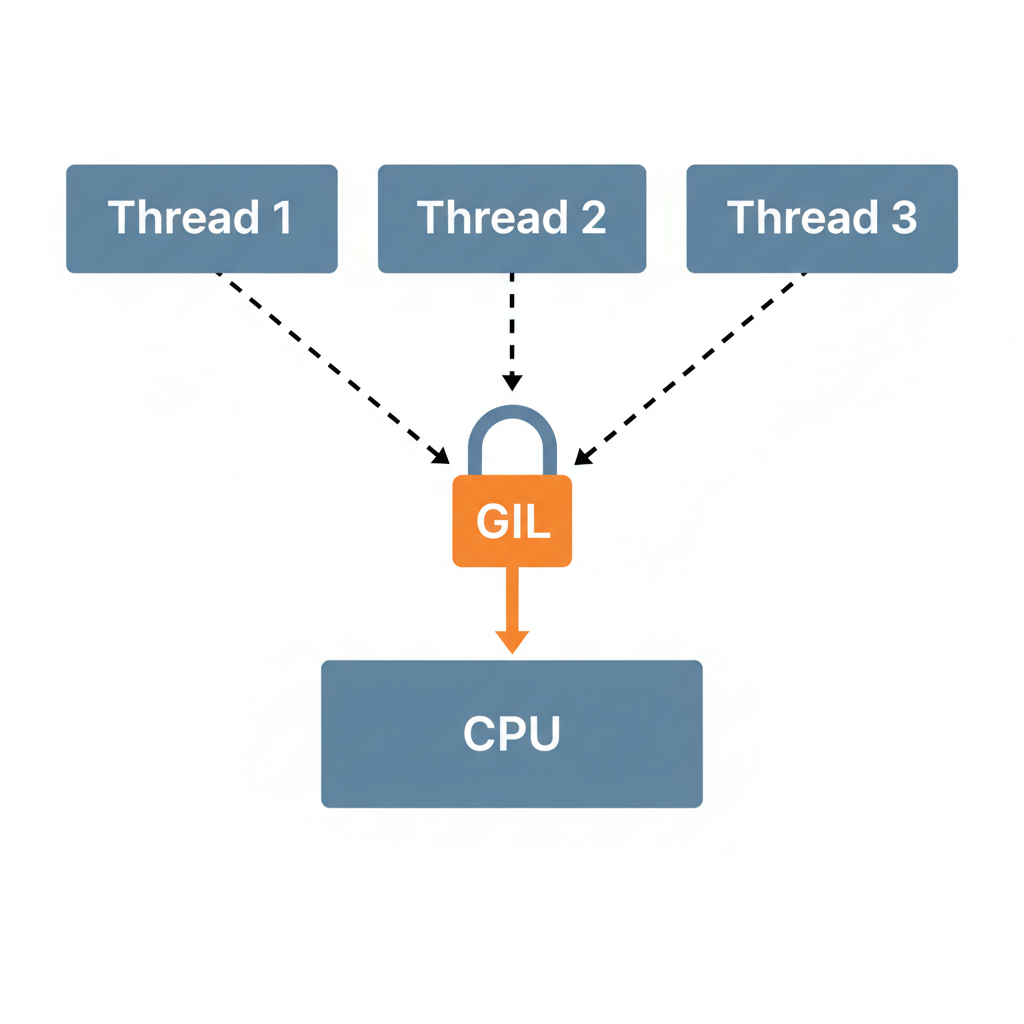
\includegraphics[height=0.6\textheight]{img/05-gil.png}
    \caption{Visualización del Global Interpreter Lock (GIL) de Python.}
  \end{figure}
\end{frame}
